\chapter{Sorting of atoms}%
\label{sec:sorting}

%\subsection*{General idea and length}

%\begin{itemize}
	%\item Give the problem, which is to study interactions, but for this we need geometries where atoms are always next to each other + idea how to solve it using aod tweezers (1 page) (I think I should explain at some point that we have slm tweezers and then would transfer into the aod tweezers)
	%\item Explain how aods work (length as is)
	%\item Setup of the aod tweezer lasers (1-2 pages)
	%\item Sorting using algorithms. Could say more about other sorting experiments. Highlight differences between sorting algorithms. (6 pages?)
	%\item I am fairly sure I should explain both algorithms in more detail
	%\item Programming the aod using the spectrum card. Explain how it works, how much memory it has and how that has an effect on the sorting algorithms. Could definitely talk more about the program that I wrote, but I don't think it's relevant. (5-6 pages)
%\end{itemize}

Tweezer arrays are especially suitable to study manybody systems, as arbitrary patterns can be configured, which is not possible when using optical lattices. In our experiment, atoms are cooled in optical molasses and loaded into tweezers in a chopping sequence, discussed in Chapter~\ref{ch:chopping}. However, in the loading stage, parity projection induces light assisted collisions of the atoms~\cite{Cooper2018}, which effectively heat pairs of atoms out of the trap. This leaves only sites occupied, that originally had odd number of atoms, resulting in a total occupation of 50\% of atoms across the tweezer array. It is desired to have a fully occupied grid of atoms each run, however post-selection is unfeasible, as even on a $3\times3$ grid of atoms, the chance of fully occupying the array is only $0.5^9 = 0.2\%$.
%Before atoms are trapped in tweezers, they are first cooled in optical molasses and are then loaded by making use of chopping. During loading,

Consequently, the solution is to rearrange the atoms of the system, which has demonstrated before~\cite{Barredo2016, Endres2016, Barredo2018}. As mentioned, the tweezers in our experiment are generated by \acp{slm}. In order to rearrange the atoms however, they need to be transferred from the static \ac{slm} tweezers, into new dynamic acousto-optically deflected tweezers. These move the atoms adiabatically to new positions, while keeping the others stationary. In this way, atoms are moved along pre-calculated paths to fill gaps of the pattern. The following chapter discusses the sorting of atoms by using \acp{aod} as the device of choice for programmatically deflecting a laser beam. Using this device, it is also possible to generate an array of tweezers, so that multiple sites at the same time can be moved.


\section{Acousto-optically deflected tweezers}

Being able to quickly change the position of a laser beam is the most fundamental prerequisite of sorting atoms. The process has to happen on short timescales compared to the lifetime of atoms and with high accuracy. As \acp{aod} can fulfill this requirement, the process of light deflecting off a sound modulated crystal is discussed in the following. By applying sound waves, it is possible to move a laser beam or split it into multiple beams. The optical element handling the deflection is called an \ac{aod} and works very similar to an \ac{aom}. However, in an \ac{aod}, the first deflected order is stronger and higher orders are generally not visible.

After going through the theory of acousto-optical deflection, the \acp{aod} in question are described, following the setup of generating the tweezers needed for the rearrangement of the atoms.

\subsection{Acousto-optical effect}

The acousto-optical effect describes the way optical waves deflect off sound waves in a solid medium, which is generally a crystal. This means, sound waves propagating the crystal modulate the positions of the atoms in the lattice, which in turn affects the refractive index on a macroscopic scale. Is the sound wave a planar wave, then the modulated refractive index is written as a function of position $x$ and time $t$~\cite{Saleh1991}:

\begin{align}
	n(x, t) = n - \Delta n_0 \cos{\left(\Omega t - q x\right)}.
\end{align}

In this case, the offset $n$ is the refractive index in absence of sound waves. Moreover, $\Delta n_0$, is the amplitude, $\Omega$ the frequency and $q$ the wavenumber given by the sound wave.

Using this relation, the next step is calculating the deflection angle off the medium. In the following, a short summary is given, the detailed analysis can be found in~\cite{Saleh1991}. Starting from the assumption that the incident optical wave has a much higher frequency than the sound wave, then the light entering the medium sees the sound waves as stationary and the medium's crystalline shape is given by the sound wave.

Then the description of light passing through a medium is given by the Bragg condition, and is used to calculate how light is partially reflected when leaving the medium. In order to calculate this quantity, the medium is broken up into slices, off which the optical wave partly reflects, given by the Bragg diffraction. Each slice has a partial reflectance amplitude $\Delta r$, depending on the refractive index $n$ and the angle of the incident optical beam with respect to the medium. The total reflectance amplitude $r$ can then be calculated by integrating over all slices and carries over the dependence on the angle. By maximizing this relation, the angle resulting in the maximum reflectance amplitude is given by the Bragg condition:

%With this relation, it is already intuitive to see, that light entering the medium will change. 
%By assuming planar optical light passing through the medium, an approach based on calculating the reflectance in the medium using Fresnel equations \cite{Saleh1991} finds that the reflectance is maximal, whenever the incident angle $\theta_B$ of the optical wave on the sound wave meets the Bragg condition:

\begin{align}
	\sin \theta = \frac{\lambda_l}{2 \lambda_s},
\end{align}

where $\lambda_l$ and $\lambda_s$ refer to the wavelength of the light and sound waves respectively.

The maximum of the reflectance amplitude with respect to the angle is very sharp, such that there is a deflected beam only if the angle between the wave vectors of the optical wave $\mathbf{k}_l$ and the sound wave $\mathbf{k}_s$ matches the Bragg condition. Thus, another way to arrive at the Bragg condition is by calculating the trigonomic relation in Figure~\ref{fig:aod_schematic}. With

\begin{align}
	\abs{\mathbf{k}_l} &= \abs{\mathbf{k}_{l,r}} = \frac{2\pi}{\lambda_l} \\
	\abs{\mathbf{k}_s} &= \frac{2\pi}{\lambda_s},
\end{align}

it follows directly, that
\begin{align}
	\label{eq:bragg_trigonometry}
	\sin{\theta} = \frac{\abs{\mathbf{k}_s} / 2}{\abs{\mathbf{k}_{l,r}}} = \frac{\lambda_l}{2\lambda_s}.
\end{align}

\begin{figure}[t]
\centering{%
\import{figures}{aod_schematic.pdf_tex}
\caption{Schematic operation of an \ac{aod}. Light waves travelling in direction $\mathbf{k}_l$ are deflected off the sound waves with direction $\mathbf{k}_s$, resulting in a reflected beam $\mathbf{k}_{l,r}$. The optical waves are deflected under the Bragg condition, which can be calculated via the vector relation $\mathbf{k}_{l,r} = \mathbf{k}_l + \mathbf{k}_s$.}%
\label{fig:aod_schematic}
}
\end{figure}

%It is now possible to exploit this acousto-optical effect in order to deflect an optical wave by an arbitrary angle. For this, the acoustic wave is modelled as a gaussian distribution of planar waves. Then the acoustic wave has planar waves travelling in every direction, such that it is always possible to fulfill the Bragg condition, independent of the angle

%Then it will always be possible to fulfill the Bragg condition, due to the fact that there is a k-vector in every direction for the sound wave.

Using the acousto-optical effect in order to modify tweezer positions, it is necessary to break the dependence of the angle between incoming optical wave and acoustic wave, while keeping the dependence on the angle of the outgoing light. This is achieved by modelling the sound wave as a Gaussian distribution of planar waves, travelling radially outwards from the origin of the sound. As a consequence of this, it will always be possible to fulfill the Bragg condition, no matter how the light enters the medium.

In Figure~\ref{fig:aod_schematic_2}, an optical beam enters a medium straight and exits on a diffracted angle $\pm \theta$, given by the Bragg condition. Using again the trigonometric relations from Equation~\ref{eq:bragg_trigonometry}, there are now additional acoustic waves travelling in opposing directions, where the optical and sound wave meet. In the approximation of small angles, the Bragg condition then simplifies to:

\begin{figure}[t]
\centering{%
\import{figures}{aod_schematic_2.pdf_tex}
\caption{Similar to Figure~\ref{fig:aod_schematic}, light is deflected off sound waves in an acousto-optical medium. This time, the sound wave is modelled as a Gaussian distribution of planar waves, such that besides the transmitted component, two more orders are deflected.}%
\label{fig:aod_schematic_2}
}
\end{figure}

\begin{align}
	\theta_\pm \approx \sin \theta_\pm = \pm \frac{\lambda_l}{\lambda_s} = \pm \frac{f_s}{v} \lambda_l,
\end{align}

where the speed of light in the medium $v$ needs to be taken into account.

This means, that the angle of the first deflected orders from the \ac{aod} only depend on the wavelengths of the light wave $\lambda_l$ and the sound wave $\lambda_s$. In other terms, the angle of deflection can be tuned by changing the wavelength of the sound wave. As the deflector is driving with an RF-generator, we generally speak of the frequency and not the wavelength of the sound wave. Using the deflector for sorting, means taking first deflected order and blocking the others.
This way, a beam can be moved by driving a frequency ramp on the sound wave, thus changing the angle of the first deflected order. Consequently, the change of angle depending on the change in frequency of the sound wave is interesting and is then calculated as:

\begin{align}
	\Delta\theta_\pm = \pm \frac {\Delta f_s}{v} \lambda_l
\end{align}%
\label{eq:aod_angle}

Thus, all parameters required for manipulating the position of laser beam have been calculated, such that the tweezers can be operated for resorting. We have seen how optical light is deflected off sound waves in media and how this can be used to re-position laser beams and in the long run, move atoms along paths. There are generally two types of \acp{aod} available, that are normal mode and shear mode. In a normal mode \ac{aom}, the shape of the crystal viewed from the top, is rectangluar, while in a shear mode, the crystal's front and back sides are cut at an angle. This means, sound waves won't be Gaussian anymore, but instead be shear waves, meaning their velocity is slower. This is in general preferable, as we made the assumption, that the speed of the sound wave is much slower than the speed of the light wave, and thus this condition is reinforced. All in all, after having understood the operation of \acp{aod}, the following chapter explains the setup in place for sorting the atoms.

\subsection{Preparation of the tweezers beams}%
\label{sec:tweezer_beams}

With the derivations from the previous chapter, it is possible to calculate the position of the laser beam, depending on the frequency of the sound wave propagating the \ac{aod}. However, the beam has to be prepared before entering the deflector, meaning its polarization has to be adjusted. After the deflector, the beam will pass an objective into the vacuum chamber and therefore needs to be shaped correctly before the objective. The setup of the laser, as well as the configuration of \acp{aod}, in order to sort in two dimensions, is described in the following.

The deflectors ((AA DTSXY-400--800.860) from Pegasus optics) and their characteristics are given in Table~\ref{tbl:pegasus_aod}. The \acp{aod} are driven by RF-frequencies, which map 1:1 to the frequency of the sound wave.  In order to deflect in two dimensions, two deflectors are placed in series, which are turned by $\SI{90}{\degree}$ with respect to each other. This way, the first order on the first \ac{aod} will extend e.g.\ into the x-axis, while the first order of the second \ac{aod} will then extend along the y-axis. Together, exiting the deflectors will be a $2\times2$ grid of laser beams, which can be seen in Figure~\ref{fig:aod_pass}. These are the $(x=0, y=0)$, $(1, 0)$, $(0, 1)$ and $(1, 1)$ orders, however, only the $(1,1)$ order will be used, as this is the one that is deflected based on the sound wave placed into the \ac{aod}.

\begin{table}[h]%
\label{tbl:pegasus_aod}
\centering
\begin{tabular}{l l}
	%\hline \hline
	\toprule \toprule
	Central drive frequency at $\SI{795}{\nano\meter}$ & $\SI{102(4)}{\mega\hertz}$ \\
	Bandwidth & $\SI{36}{\mega\hertz}$ \\
	Max optical power density & $\SI{5}{\watt\per\milli\meter\squared}$ \\
	Max RF power & $\SI{2}{\watt}$ \\
	Laser beam diameter [$D$] & $\SI{500}{\micro\meter}$ < D < $\SI{6}{\milli\meter}$ \\
	Material (speed of sound) & TeO2 ($\SI{650}{\meter\per\second}$) \\
	Scan angle & ${(\SI{44}{\milli\radian})}^2$ \\
	\bottomrule \bottomrule
\end{tabular}
\caption{Properties of AA DTSXY-400--800.860 crossed \acp{aod} from Pegasus optics.}
\end{table}

\begin{figure}[ht]%
\centering{%
\import{figures}{aod_pass.pdf_tex}
\caption{Light passing through two \acp{aod} is deflected into a 2-dimensional grid. The colors refer to the optimized power going into the respective order, from lightest color being lowest power to darkest color being highest power. This way, the least amount of power goes into the (0,0) order and most into the (1,1) order.}%
\label{fig:aod_pass}
}
\end{figure}

The details of the configuration and characterization of the devices used in the experiment are given in~\cite{Osterholz2020}. The crossed \acp{aod} configuration described above is used in the following for rearranging the atoms. Additionally, the dynamic tweezers generated from the deflectors are also used for a spin-selective imaging approach, which is further described in Chapter~\ref{ch:spin_resolved}. This means, beam paths of two different lasers are passing through the same deflectors. In Figure~\ref{fig:setup_aod}, the setup including both laser beams is shown. The first laser, used for the characterization in~\cite{Osterholz2020} and later sorting of atoms, as well as for testing reasons regarding the tweezers in the following and has a wavelength of $\SI{795}{\nano\meter}$. The spin-selective laser has a wavelength of $\SI{768}{\nano\meter}$ and is further discussed in Chapter~\ref{ch:spin_resolved}.

\begin{figure}[t]%
\centering
\import{figures}{setup_aod.pdf_tex}
\caption{Beam path to generate acousto-optically deflected tweezers. Two beams used for sorting and spin-resolved imaging are combined using a \ac{pbs}. They pass the \ac{aod} after which the beam is shaped to match the objective into the experimental chamber.}%
\label{fig:setup_aod}
\end{figure}

The first step in the setup, is stabilizing the intensity of laser beams, by measuring their power on a photodiode and using proportional-integral controllers to adjust the signal. They then pass a $\lambda/2$ waveplate to adjust the polarization, which affects the efficiency of the \ac{aod}. The deflectors, which are connected to RF-synthesizers, then produce the $2\times2$ grid of laser beams. Afterwards, a $f=\SI{75}{\milli\meter}$ lens, projecting the center of the \ac{aod}-array, extends the beam spatially until it is collimated using a $f=\SI{1000}{\milli\meter}$ lens. This sets the correct beam size for the objective to project the beam onto the atoms.

\subsection{Moving tweezers}%
\label{sec:moving_tweezers}

It was shown, how the position of the laser is calculated using the Bragg condition in Equation~\ref{eq:aod_angle}. With the laser setup in place, the question remains how the change of the sound wave frequency affects the position of the tweezer in the plane of the atoms. This is calculated, by taking into account the magnification $M$ due to the telescope created between the $f=\SI{1000}{\milli\meter}$ lens and the objective, having an effective focal length of $\SI{33.18}{\milli\meter}$. From the point of view of the atoms, this results in $M=\frac{1000}{33.18} = 30.14$, meaning the distance between the atoms $\Delta x$ is magnified by this amount. Continuing from the atom's reference frame, their magnified distance is then given on the $f=\SI{75}{\milli\meter}$ lens as a distance $\Delta x_{magnified} = Mx$, which projects the position into the center of the crossed \ac{aod} configuration at an angle $\tan{\theta} \approx \theta = \Delta x_{magnified} / \SI{75}{\milli\meter}$.
With Equation~\ref{eq:aod_angle}, this results in a change of frequency on the \ac{aod}:

\begin{align}
	\Delta f = \frac{\Delta x_{magnified}}{\SI{75}{\milli\meter}} \frac{v}{\lambda},
\end{align}

given an optical laser wavelength of $\lambda$. The speed of sound for the \acp{aod}, which is the speed of sound in $\ce{TeO2}$ is $v=\SI{650}{\meter\per\second}$. This means a typical atomic distance of $\SI{10}{\micro\meter}$, requires a change in frequency of $\Delta f = \SI{3.3}{\kilo\hertz}$.

\subsection{Tweezer homogeneity}

With all the building blocks in place, for driving acousto-optically deflected tweezers, they are now ready to be imaged and tested. The beam path shown in Figure~\ref{fig:setup_aod} was used, except the objective at the very end was replaced by an $f=\SI{500}{\milli\meter}$ lens and a camera (XIMEA MD028MU-SY). This way, the tweezers are visible directly on the camera. Moreover, in order to measure the homogeneity more accurately, part of the beam is split and coupled into a photodiode after the $f=\SI{500}{\milli\meter}$ lens. This way, an image was taken with a camera and at the same time, a trace was taken from the signal of the photodiode. Although it is technically possible, to draw a grid with the \acp{aod}, by applying a superposition of multiple frequencies, the measurement discussed in the following was taken by turning on each tweezer separately one after another. This way, they can be distinguished powerwise.

The Figures~\ref{fig:aod_grid} and~\ref{fig:aod_hom} show the results of these measurements. It can be seen in the camera image, that there is a slight field of view effect in the top-left corner. The order of activation of the tweezers was to start in the lower right hand corner, continuing to the left and after row-wise towards the top. This allows to map them back to the intensity seen in the oscilloscope picture. The oscilloscope also shows an intensity ramp towards the end, which suggests the same field of view and therefore being an effect of the beam not perfectly aligned. Nonetheless, the intensity difference between the first and last set of tweezers is about $\SI{0.1}{\volt}$ or $5\%$ when the distance between lattice points was given by a frequency difference $\SI{1}{\mega\hertz}$. However, as noted in Section~\ref{sec:moving_tweezers}, this is higher by almost a factor of 1000, suggesting that the tweezer homogeneity will be much higher once integrated into the experiment.

\begin{figure}[t]%
\centering
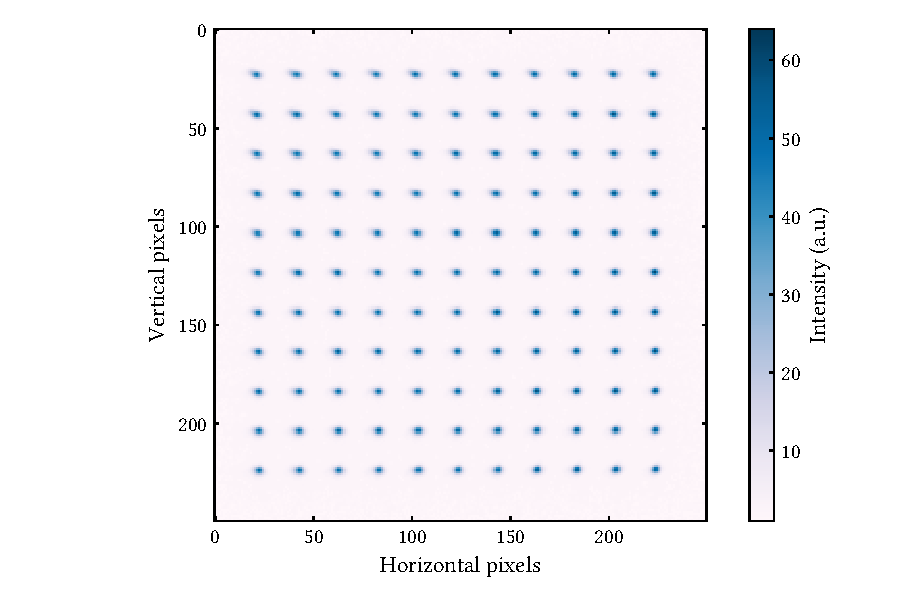
\includegraphics{figures/aod_grid_155.pdf}
\caption{An image of tweezers was acquired by activating a set of $11\times11$ frequency combinations on the crossed \acp{aod}. A slight field of view effect is visible in the top-left corner.}%
\label{fig:aod_grid}
\end{figure}

\begin{figure}[t]%
\centering
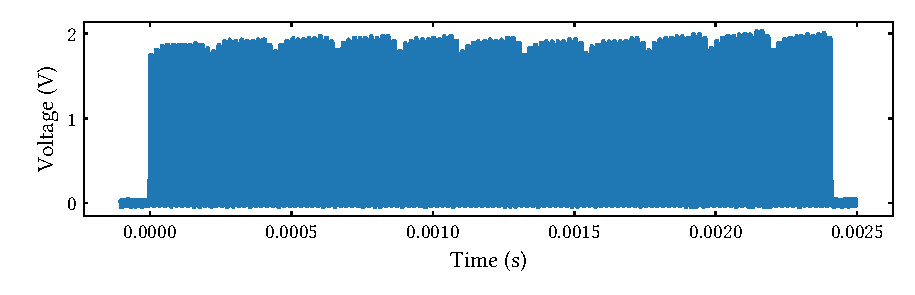
\includegraphics{figures/aod_hom_155.pdf}
\caption{The same tweezer picture as in Figure~\ref{fig:aod_grid} was acquired using a photodiode. There is a trend of intensities growing towards the later tweezers. Between the last set of tweezers and the first, the difference is about $\SI{0.1}{\volt}$ or $5\%$.}%
\label{fig:aod_hom}
\end{figure}

\section{Sorting algorithms}

With the laser now passing through the crossed \acp{aod} and being shaped for the objective, it is time to rearrange the atoms for the experiment. Doing so requires the knowledge about unloaded \ac{slm} tweezers, which is achieved by imaging the atoms and evaluating their posstions. Of course, atoms can't be lost during imaging, therefore cooling and trapping beams are chopped together and the scattered light from the cooling beam is recorded as a fluorescence image. From then on, atoms need to be moved along paths in order to fill the gaps. They can be lost, if the move is on the order of the scattering rate, as then the trap moves out of range while an atom is in the excited state. Generally speaking, the move needs to be as fast as possible, since heating effects discussed in Chapter~\ref{ch:chopping} lead in our experiment to $1/e$ lifetimes on the order of 80 seconds. Therefore, already $1.2\%$ of atoms, or at least one atom in a $10\times10$ grid are lost after one second.

Sorting the atoms as fast as possible in order to reach $100\%$ filling requires paths that minimize the total sorting time. An obvious choice here is Dijkstra's algorithm, wich is designed to find the minimal path between two points, in an arbitrary landscape. However, since the paths have to be calculated while the atoms are loaded, this means computation complexity has to be taken into account as well. Since Dijkstra's algorithm scales with $\mathcal{O}(n^4)$\docite{}\todo{ref}, where $n$ is the number of atoms, this can lead to long computation times. However, some simplifications can be made, which can help come up with an algorithm that is both fast in calculation speed, as well as having fast sorting speeds.
For one, we are operating on a rectangular grid and thus make the simplification to only move vertically or horizontally and not diagonally. Secondly, atoms that have started moving, stay in the tweezer until they arrive at their destination, and thus the tweezer does not suddenly jump to a new target. This is a sensible simplification, as an atom has to be transferred from the initial tweezer array to the moving tweezers (and back again when it arrives at the destination), which also takes up time. In the description of the algorithms, the grid is separated into a target and a reservoir region. This means we are trying to get a $100\%$ filling in the target region, by moving atoms out of the reservoir region. Any atoms left in the reservoir after the sorting is finished, will be discarded. On the other hand, while there are still holes in the target region, the algorithm will look for ways to fill the gaps using atoms from the reservoir region.

Two algorithms (pathfinding and compression) are presented in the following, one is based on solving a pathfinding problem and moves one atom at a time. The other uses the feature of the \ac{aod}, that allows to work move several tweezers at once, by applying multiple RF frequencies, in order find a more parallelized approach.


\subsection{Pathfinding}

The pathfinding problem is solving the problem of finding the shortest path between two points. For sorting of atoms, this means identifying the shortest set of movements to relocate an atom from the reservoir region to an empty spot in the target region.
The algorithm described in the following was developed by Jan Werkmann\footnote{https://github.com/PhyNerd/GridRouting} and is discussed in~\cite{OhldeMello2020}. With the simplifications of above, atoms only move either horizontally or vertically. The algorithm will then identify a path that first moves the full distance of the one dimension, then the full distance in the other, at which point the atom has arrived at its destination. This is a sensible approach, as only one frequency ramp per dimension is driven, but does not change the total distance moved, since the atom won't move on diagonals.
Then there are only two possible paths every atom can take, either going first vertically then horizontally, or the other way around. The optimal path is then the one with the least amount of atoms in it. If there happens to be an atom in the path, the algorithm segmentizes the path, moving the obstacle atom along the path into the unoccupied spot, with the other atom following after. An example path is shown in Figure~\ref{fig:sorting_path}.

\begin{figure}[tbp]%
\centering
\import{figures}{sorting_path.pdf_tex}
\caption{Conceptual illustration of the pathfinding algorithm for resorting. The atom tries to move into a hole but has an obstacle (which is just another atom) in its way. The obstacle is first moved out of the way, after which the atom follows. The target area is then further filled with the remaining atom.}%
\label{fig:sorting_path}
\end{figure}

\subsection{Compression}%
\label{sec:compression}

As was just discussed, the pathfinding algorithm moves atoms one by one. However, one might want to find a way to parallelize sorting, therefore decreasing the sorting time. By supplying an \ac{aod} with multiple RF-frequencies, it is possible to create multiple movable tweezers. The compression algorithm discussed here makes use of this in order to reduce the total time of the sorting, as well as having a lower computation time with respect to the pathfinding algorithm.

The compression algorithm works by picking a full line of atoms. It then moves the selected atoms along the line towards the target area, grid point by grid point. If an atom would collide with an obstacle, that is, either another atom not currently inside an \ac{aod} tweezer, or the end of the target area, then that atom is transferred back to the \ac{slm} tweezer grid, and not moved in the next step. This process is shown in~\ref{fig:sorting_compression}. When one line is finished moving according to this end condition, the next line is picked up and the process repeated. This is done first for all rows, then for all columns, and finally, all atoms are found in one corner of the grid. Doing it this way, effectively compresses all atoms in the grid into an area.

\begin{figure}[tbp]%
\centering
\import{figures}{sorting_compression.pdf_tex}
\caption{Sorting atoms using the compression algorithm is done by selecting a full line of atoms. They are then moved towards the left edge. An atom that meets the edge is released before the others continue moving. When the steps for the rows have are completed, the same process follows for the columns.}%
\label{fig:sorting_compression}
\end{figure}

Due to the nature of the algorithm, there can still be holes in the target area when the sequence is finished. To overcome this problem, following the compression stage, the pathfinding algorithm will fill the final few gaps, whose runtime is favorable towards low hole numbers.

To further take advantage of the compression algorithm, a geometry is chosen, which has the target area in the center of the grid and the reservoir surrounding it, as seen in Figure~\ref{fig:sorting_compression}. As the algorithm pushes the atoms into a corner, the grid can simply be split up into four sections. Then the moves for each section is individually calculated. Ending up with moves in the row-dimension and moves in the column-dimension for each section, they can then be merged together, if they operate on the same line, which is illustrated in Figure~\ref{fig:compression_split}. As such, the sorting time of moving atoms into one corner is effectively the same as moving the atoms into the central area, by splitting it up into sections and merging the steps.

\begin{figure}[tbp]%
\centering
\import{figures}{compression_split.pdf_tex}
\caption{Sequence of finding parallelized paths for the compression algorithm. Since atoms are always sorted into a corner, the compression algorithm can be split into four sections. The compression is run over each section, which finds the paths to move the atoms into a corner. In the last step, all paths that are in the same row or column, are combined and thus parallelized.}%
\label{fig:compression_split}
\end{figure}

\subsection{Comparison of the two algorithms}

As the pathfinding and compression algorithm are both solving the same sorting problem, it is necessary to make a performance comparison between the two. For the simulation of the performance comparison, the target area was chosen to be in the center, surrounded by the reservoir region. This gives a geometry, which has holes as close as possible to reservoir atoms, therefore giving a minimal number of movements for the pathfinding algorithm, while also making use of the performance gain that was highlighted in Section~\ref{sec:compression} for the compression.

Relevant parameters that need to be compared, are the sorting and computation time, as they need to be much slower than the lifetime of the atoms. Atom loss can also occur, whenever the atoms are transferred from the \ac{slm} tweezer grid to the \ac{aod} tweezer grid used for the sorting. This way, the number of transfers are also shown in the following.
Simulations were performed, by populating the full grid with atoms with $\SI{50}{\percent}$ probability of occupying a grid point. Then each algorithm was run and relevant parameters recorded. Simulations were run for various grid sizes, while trying to keep the fraction of number of atoms in the target area $N_{target}$ to the number of atoms in the reservoir area $N_{reservoir}$ around $\frac{N_{target}}{N_{reservoir}} \approx 0.65$. This has to be compromised for low grid sizes, as the integer nature of grid points only allows natural numbers for reservoir sizes.

The results in Figure~\ref{fig:sorting_algos} show that the compression algorithm has a faster sorting and computation time, but has to transfer more atoms into the \ac{aod} tweezer grid. However, it also shows that it scales better for increasing grid sizes. A polynomial fit is shown for the second half of the points, where the rounding issue is less present. The fit parameters are given in Table~\ref{tbl:sorting_algo_fit}, from where it can be seen, that the compression algorithm scales more linearly than the pathfinding algorithm.

\begin{figure}[tbp]%
\centering
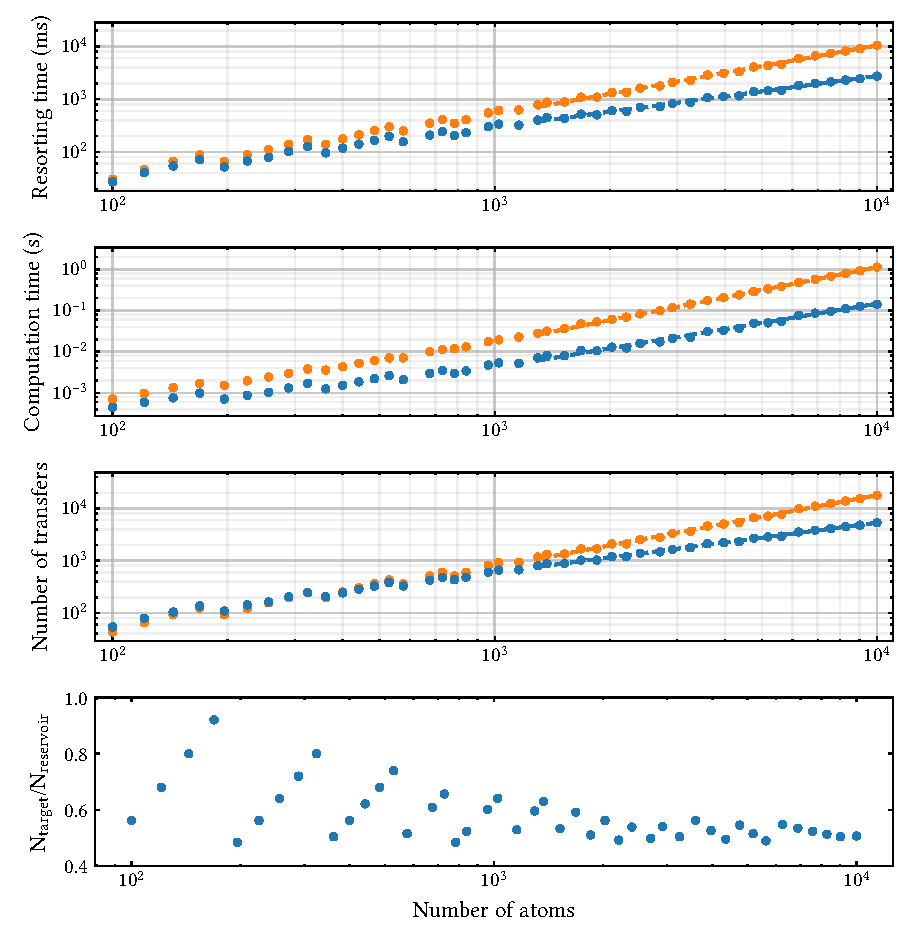
\includegraphics{figures/sorting_algos_155.pdf}
\caption{Comparison of pathfinding algorithm (orange) and compression algorithm (blue) for sorting atoms into a target region. For each data point, 50 simulations were run and the mean of the result is shown. Standard deviation is on the size of the dots drawn and as as such are not visible. The fraction of atoms in the target versus the reservoir area are shown in the last diagram. Since only integer values are allowed for the reservoir size, the fraction between the two sees a rounding effect. For this reason, the fit is only done for the upper half of the data points, where the effect is less pronounced. The values to the fit are given in Table~\ref{tbl:sorting_algo_fit}.}%
\label{fig:sorting_algos}
\end{figure}

\begin{table}[ht]%
\label{tbl:sorting_algo_fit}
\centering
\begin{tabular}{l l l}
	\toprule \toprule
	\multicolumn{3}{c}{Pathfinding} \\ \thickhline{}
	& $m$ & $a$ $(ms)$ \\ \midrule
	Resorting time & \num{1.3e+00} $\pm$ \num{1.7e-02} & \num{5.8e-02}  $\pm$ \num{8.8e-03} \\ \midrule
	Computation time & \num{1.8e+00}  $\pm$ \num{8.9e-03} & \num{4.8e-05}  $\pm$ \num{3.8e-06} \\ \midrule
	Number of transfers & \num{1.4e+00}  $\pm$ \num{1.8e-02} & \num{5.7e-02}  $\pm$ \num{9.2e-03} \\ 

	\midrule \midrule
	\multicolumn{3}{c}{} \\
	\midrule \midrule
	\multicolumn{3}{c}{Compression} \\ \thickhline{}
	& $m$ & $a$ $(ms)$ \\ \midrule
	Resorting time & \num{9.7e-01} $\pm$ \num{1.7e-02}  & \num{3.6e-01} $\pm$ \num{5.3e-02}  \\ \midrule
	Computation time & \num{1.6e+00} $\pm$ \num{3.1e-02}  & \num{9.0e-05} $\pm$ \num{2.5e-05}  \\ \midrule
	Number of transfers & \num{9.5e-01} $\pm$ \num{1.2e-02}  & \num{8.3e-01} $\pm$ \num{8.6e-02}  \\ \midrule
	\bottomrule
\end{tabular}
\caption{Comparison of scaling of the two sorting algorithms. For each quantity given in the left-most column, a polynomial $f(x) = aN^m$ was fitted to the points shown in Figure~\ref{fig:sorting_algos}. This gives $m$ as the scaling and the parameter of interest, resulting in better scaling in every aspect for the compression algorithm.}
\end{table}

\section{Driving an RF-synthesizer for arbitrary pattern generation}

One of the most powerful aspects about \acp{aod} is the fact, that a superposition of sound waves results in a superposition of light waves in the output. This way, it is possible to generate a grid of tweezers, by supplying each \ac{aod} with one or more RF-frequencies. There are a multitude of ways to generate RF-frequencies, one way is using \acp{vco}, which can be simple LC-circuits. Using these, it is also possible to drive frequency ramps, however it is not possible to synthesize multiple frequencies from one \ac{vco}, meaning it is necessary to use multiple \acp{vco} together. Therefore using this approach it is possible to sort the atoms one-by-one, however it is not possible to generate grid patterns.

To overcome this issue, we implement a digitizer card (M4i.6600-x8, Spectrum Instrumentation), whose specifications are summarized in Table~\ref{tbl:spec_m4i}. Doing so allows to sample arbitrary signals, for example sines, rectangles or even non-periodic ones. A \ac{dac} on the board converts the sampled points into an analog signal, which can be passed into the \ac{aod}.

\subsection{Functionality of the Spectrum driver}

Communication with the card is provided through a low-level interface from the official drivers over a PCIe slot. In the following, two replay modes of the spectrum card are discussed, which are standard replay mode and sequence replay mode. In single replay mode, a signal is sent onto the card, which is played back a set number of times, from start to finish. The sequence replay mode allows to upload sequences during initialization. It is then possible to play any arbitrary combination of the sequences one after another.

\begin{table}[tbp]%
\label{tbl:spec_m4i}
\centering
\begin{tabular}{l l}
	\toprule \toprule
	Maximum sampling rate & $\SI{1.25}{\giga\samples\per\second}$ \\
	Output level (at max sampling rate) & $\pm \SI{4}{\volt}$ \\
	Transfer speed PC to card & $\SI{2.8}{\giga\byte\per\second}$ \\
	Memory & $\SI{4}{\giga\byte}$ \\
	\bottomrule \bottomrule
\end{tabular}
\caption{Relevant parameters of the Spectrum M4i.6600-x8 card from the specifications given by the manufacturer.}
\end{table}

The functionality of the card depends on two factors: The layout of the memory, and the readout speed (the sampling rate) of the memory. In the following implementation, two output channels of the spectrum card are used. Doing so, the memory is formatted, such that two bytes of channel 1 data are followed by two bytes of channel 2 data as seen in Figure~\ref{fig:spectrum_memory}. Transferring data onto the memory then requires to fill a buffer, that is, memory on the computer running the driver, that has the same layout as the spectrum card's memory.
\begin{figure}[tbp]%
\centering
\import{figures}{spectrum_memory.pdf_tex}
\caption{Sampled data points are stored in a local buffer, which can then be transferred into the cards memory. The memory is effectively 1-dimensional, with two bytes for each sampled data point. Example signals are given for Channel 1 (red) and Channel 2 (blue). In the single replay mode, the data pointer will read from the first memory position until a given end point. In sequence replay mode, the data pointer will move forward, but can jump at any point based on user preference.}%
\label{fig:spectrum_memory}
\end{figure}

With this information, the structure of a program driving the digitizer card follows the format given in Table~\ref{tbl:replay_modes}.

\begin{table}[tbp]%
	\label{tbl:replay_modes}
	\centering
	\begin{tabular}{p{0.2\textwidth} p{0.7\textwidth}}
		\midrule \midrule
		&
		Single replay mode \\
		\thickhline%
		Initialization phase &
		\begin{tabular}[c]{@{}p{0.7\textwidth}@{}}\tabitem{} Set sampling rate\\ \tabitem{} Set replay mode to single replay mode\\ \tabitem{} Allocate the buffer memory\end{tabular} \\
		\midrule
		Main loop &
		\begin{tabular}[c]{@{}p{0.7\textwidth}@{}}\tabitem{} Sample datapoints of the signal to play and move into the buffer\\ \tabitem{} Transfer datapoints from the buffer to the card\\ \tabitem{} Replay signal $N$ times\end{tabular} \\
		\\
		\bottomrule \bottomrule
		&
		Sequence replay mode \\
		\thickhline%
		Initialization phase &
		\begin{tabular}[c]{@{}p{0.7\textwidth}@{}}\tabitem{} Set sampling rate\\ \tabitem{} Set replay mode to sequence replay mode\\ \tabitem{} Sample signals to use in the sequence programmed later\\ \tabitem{} Transfer signals onto the card\\ \tabitem{} Allocate the buffer memory (will contain information about the sequence)\end{tabular} \\
		\midrule
		Main loop &
		\begin{tabular}[c]{@{}p{0.7\textwidth}@{}}\tabitem{} Fill buffer with information about which signals to play\\ \tabitem{} Transfer buffer to the card\\ \tabitem{} Play sequence\end{tabular} \\
		\bottomrule \bottomrule
	\end{tabular}
	\caption{Difference in programming when using either the single replay or the sequence replay mode of the Spectrum M4i card. In this case, it is instructive to see, that the single replay mode has an overhead during the main loop compared to the sequence replay mode, which has all sequences stored in memory already.}
\end{table}

The maximum transfer speed for transferring data from the PC to the spectrum card is $\SI{2.8}{\giga\byte\per\second}$, this means that it will always be preferrable to move as few data as possible. Consequently, if possible, it is advantageous to use the sequence replay mode, as here, almost all data is already transferred in the initialization phase. All that is left to transfer, is the sequence the data pointer is following.

\subsection{Limits of using the card in the experiment}

There are some considerations to make when using a digitizer card as a driver for acousto-optical tweezers. Since the digitizer replays sampled data points from waveforms, this means data points need to be transferred from a computer memory to the digitizer card. The transfer time should of course be kept minimal, since the information about which wafeforms to sample is only available when atoms are already loaded into tweezers and their lifetime in the tweezer traps is finite (on the order of $\SI{80}{\second}$ for our experiment). Transferring data points to the spectrum card can be done in advance in the sequence replay mode, however this requires the internal memory of the digitizer to be big enough to hold all possible waveforms to be replayed. Both the transfer time and memory usage are calculated in the following, considering both the standard replay mode and the sequence replay mode.
%The first is, that the transfer of the data onto the card takes time and is given by the transfer speed. This means, that transferring data onto the card while atoms are loaded can be problematic, if the transfer time is on the order of the lifetime of the atoms, since that means that atoms are lost during this time. This can be solved by making use of the sequence replay mode, however to make use of this mode means that a large amount of memory needs to be available on the card.

In order to calculate the transfer time and memory usage, some assumptions need to be made. The assumptions and all necessary variables are summarized in Table~\ref{tbl:spectrum_assumptions}. First of all, the central frequency of the AOD is approximately $f_{AOD} = \SI{100}{\mega\hertz}$. Therefore, in order to sample a sine at this frequency with at least 10 points per oscillation, means a sampling rate of at least $\SI{1}{\giga\samples\per\second}$. For the M4i digitizer card, this means the next available setting is $\SI{1.25}{\giga\samples\per\second}$ and gives about 13 samples per oscillation. Being able to resolve the signal clearly, has the advantage to generate the frequency more accurately, therefore the $10$ samples per oscillation is a good limit.

\begin{table}[tb]%
\label{tbl:spectrum_assumptions}
\centering
\begin{tabular}{l l}
	\toprule \toprule
	Variable & Used or assumed value \\ \thickhline%
	Sampling rate & $\SI{1.25}{\giga\hertz}$ \\
	Central \ac{aod} driving frequency & $\SI{100}{\mega\hertz}$ \\
	Adiabatic transfer time to new grid & $\SI{1}{\milli\second}$ \\
	Adiabatic movement time to next grid point & $\SI{1}{\milli\second}$ \\
	Grid size & $10\times10$ \\
	Number of tweezer transfers for sorting & 60 \\
	Number of movements for sorting & 40 \\
	\bottomrule \bottomrule
\end{tabular}
\caption{Variables and assumptions used in the calculations for estimation of data transfer time and memory usage under the consideration of the experiment discussed in this thesis.}
\end{table}

Now in order to calculate the time to transfer an atom adiabatically from the \ac{slm} tweezer grid into the \ac{aod} tweezer grid (and back again), the relation $\dot{w} > w^2$ needs to be fulfilled, where $w$ is the trap frequency in transverse direction. The following argumentation follows the directions in~\cite{Leseleuc2018}. In our case, this is on the order of $\SI{20}{\kilo\hertz}$ and is fulfilled for a transfer time of $t_{transfer} = \SI{1}{\milli\second}$. In order to calculate the moving time $t_{move}$ for an atom from one grid point to another, the shape of the trap is considered. If the atom is accelerated in the first half of the movement, and decelerated in the second half of the movement, the total distance to transfer the atom is given as $L=a t_{move}^2$. The maximal acceleration is found from the trap waist $w = \SI{1}{\micro\meter}$ and its radial frequency $f_{rad} = \SI{100}{\kilo\hertz}$, as $a_{\max} \approx w f_{rad}^2 = 10^4\SI{}{\meter\per\second\squared}$. Therefore, choosing a conservative acceleration $a=\SI{10}{\meter\per\second\squared}$ results in a moving time $t_{move} = \SI{1}{\milli\second}$ over a distance $L=\SI{10}{\micro\meter}$.

With the transfer time, moving time, and sampling rate in place, the size of one signal, in order to move and transfer an atom, can be calculated as:

\begin{align}
	n_{points} &= S t = \SI{1.25}{\giga\samples\per\second} * \SI{1}{\milli\second} = \num{1.25e6} \\
	M_{sig} &= \SI{2}{\byte} * n_{points} = \SI{2.5}{\mega\byte},
\end{align}

where $\SI{1}{\byte}$ is one byte and $t=T_{move}=t_{transfer}$. From the simulations of the algorithms in Figure~\ref{fig:sorting_algos}, we see that assuming a $10\times10$ grid, there are about 60 tweezer transfers and 40 movements for one sorting. This means 100 sequences need to be played per channel, which is $n_{seq}=200$ in total. Lastly, the memory for all signals needs to be aligned to a power of two. Therefore, from the transfer speed $v_{transfer}$ in Table~\ref{tbl:spec_m4i} follows the time it takes for one transfer $t_{transfer}$:

\begin{align}
	t_{transfer} = \lceil n_{seq} M_{sig}\rceil_2\, v_{transfer} = \SI{183}{\milli\second},
\end{align}

where the symbol $\lceil \ldots \rceil_2$ refers to rounding up to the next power of two.
These calculations set the limit for the single replay mode, however, in the sequence replay mode, the limiting factor is the memory it takes to store all possible sequences. The storage of the sequences already assumes knowledge of the composition of both channels. Therefore it is necessary to upload every relevant combination of signals for both channels. Working again with a $10\times10$ grid of atoms, all relevant signals are found from the following table:

%\begin{table}[h!]%
\begin{center}
\begin{tabular}{l l l}
	\toprule \toprule
		Signals on channel 1 & Signals on channel 2 & Usage \\ \thickhline%
		10 intensity ramps up & 10 intensity ramps up & Transfer into \ac{aod} grid \\
		10 intensity ramps down & 10 intensity ramps down & Transfer out of \ac{aod} grid \\
		9 frequency ramps up & 10 constant frequencies & Move along x-axis \\
		9 frequency ramps down & 10 constant frequencies & Move along x-axis \\
		10 constant frequencies & 9 frequency ramps up & Move along y-axis \\
		10 constant frequencies & 9 frequency ramps down & Move along y-axis \\
	\bottomrule \bottomrule
\end{tabular}
\end{center}

Therefore, by multiplying the signals in the columns and then adding the rows, there are 560 combinations and $n_{seq} = 560*2=1120$ signals to upload onto the card. Each having a size of $M_{sig} = \SI{2.5}{\mega\byte}$ results in a required memory of $M_{req}=\SI{2.8}{\giga\byte}$. More generally, on a NxM grid, the number of sequences can be calculated via
\begin{align}
	n_{seq} = 2 N M + 2 N (M-1) + 2 (N-1) M
\end{align}

and therefore the required memory is
\begin{align}
	M_{req} = \SI{5}{\mega\byte} * n_{seq}.
\end{align}

With the calculations above, it is possible to apply the pathfinding sorting algorithm to the atoms in a timely manner. However for the compression algorithm, a much larger amount of signals needs to be sampled to cover all possible combinations. Considering, that two sides of the target area are sorting at the same time, and that slices of one row (or column) is selected at the same time, the number of sequences, in one channel, to move one row is then given by
\begin{align}
	n_{seq,row} = {\left(\sum_{N=1}^{M-1} N\right)}^2 = \frac{1}{4} {(M^2-M)}^2.
\end{align}

The square comes frome the fact, that for every frequency ramp on one side, a frequency ramp on the other side of the target area needs to be matched. A similar relation (replacing $M$ by $N$) is found for the number of sequences for the columns. Then, considering that the channels aren't independent, the total number of sequences is found by:

\begin{align}
	n_{seq} = M n_{seq,col} + N n_{seq,row}.
\end{align}

Taking also into account, that after the compression phase follows a pathfinding phase, it is already easy to see, that the memory requirement would greatly exceed the available memory of $\SI{4}{\giga\byte}$ on the spectrum M4i on a $10\times10$ grid.

This means, in order to use the compression algorithm, the sequences need to be sample on-the-fly. This is in general slow, compared to the sorting time. However, it is possible to use parallelization of \acp{gpu}. On a NVIDIA Geforce GTX 1080 Ti, 3584 cores are available, which can all sample part of a signal individually. This means for a sequence of $\SI{5}{\mega\byte}$, $\SI{2}{\byte}$ per datapoint, about 700 calculations are made in parallel. Assuming only rectangles are sampled, this gives one comparison per sampled value and one insertion (into an array). At a clock speed of $\SI{1480}{\mega\hertz}$~\cite{NVIDIA}, results in $\SI{0.5}{\micro\second}$ computation time, meaning only transfer speed from the \ac{gpu} to the digitizer card is relevant. The transfer speed is then given from Table~\ref{tbl:spec_m4i}, adding $\SI{1.8}{\milli\second}$ per move of one row (or column) of atoms.

Since one channel always has a fixed frequency, it is possible to use a \ac{vco} for the this channel, meaning only half of the signals need to be sampled.

\section{Conclusion}

It was shown how crossed \acp{aod} are used, in order to generate movable tweezers. As loading of atoms can only guarantee 50\% filling, the tweezers are then used to sort atoms into the gaps, in order to guarantee a perfectly occupied grid, as long as the sorting happens faster than the lifetime of the atoms. Two different algorithms were discussed that move the atoms to their new locations, which are a pathfinding algorithm, moving single atoms and a compression algorithm, which is able to use parallelization, such that multiple atoms are moved at the same time. It was shown that this approach reduces computation time of paths and sorting time of the atoms. Lastly, it was explained how the signals are generated using a digitizer card and the memory requirement for both algorithms were stated. It was shown, that as long as the grid is small enough, the pathfinding algorithm can be used with the digitizer card, as it has a smaller memory footprint. However, for a grid size of $12\times12$ already, the memory of the digitizer card (Spectrum M4i.6680-x8) is not sufficient, such that on-the-fly calculations are inevitable and the compression algorithm, with smaller computation time, can be used.
